\chapter{Ansible}
\label{chap:Ansible}

\section{关于Ansible}
\label{sec:AboutAnsible}

Ansible是一款自动化IT工具。它可以配置系统、部署软件、编排更复杂任务,诸
如连续部署或零停机滚动更新。

Ansible使用SSH协议进行通信。它是无客户端的工作方式,被管理端只需要存
在SSH客户端即可。

\begin{figure}[hbtp]
  \centering
  
\includegraphics{graph/network01.pdf}
  \caption{网络七层模型}
\end{figure}

\section{安装Ansible}
\label{sec:InstallAnsible}

Ansible的安装很简单,配置好EPEL源后,就可以直接使用yum来进行安装了。

\begin{verbatim}
yum install -y ansible
\end{verbatim}

\section{测试Ansible}

确定我们的ansible可以正常使用,接下来,我们准备几台测试机器。由
于ansible是无agent的配置管理工具,在客户端无需安装任何额外程序,使
用SSH协议进行通信,而SSH是默认安装的。

为了今后方便进行配置管理,我们需要使用SSH无密码进行通信。本测试的几台主
机及主机名为:

\begin{table}[!ht]
  \centering
    \begin{tabular}{ll}
      \toprule
      主机           & 说明   \\
      \midrule
      192.168.56.150 & 主控端 \\
      192.168.56.111 & 被控端 \\
      192.168.56.112 & 被控端 \\
      \bottomrule
    \end{tabular}
    \caption{Ansible测试环境}
    \label{tab:AnsibleTestEnv}
\end{table}

在主控端生成SSH密钥对,并把公钥分发到被控端的机器上。
\begin{verbatim}
# ssh-keygen -t rsa
# ssh-copy-id -i /root/.ssh/id_rsa.pub root@192.168.56.111
# ssh-copy-id -i /root/.ssh/id_rsa.pub root@192.168.56.112
\end{verbatim}
以上配置完毕,我们来简单的使用一下。比如,ping测试一下我们的被控端是否
存活。
\begin{verbatim}
# cat /etc/ansible/hosts
[my1]
192.168.56.111
192.168.56.112

# ansible my1 -m ping 
192.168.56.111 | success >> {
    "changed": false, 
    "ping": "pong"
}

192.168.56.112 | success >> {
    "changed": false, 
    "ping": "pong"
}

命令说明:
   my1 -- ansible操作的对象,my1组里有2台机器
   -m  -- 表示使用的是ansible的哪个模块,默认是command模块
\end{verbatim}
\subsection{command模块}
\label{sec:AnsibleCommandMod}

使用command模块,可以执行一些比较简单的命令。command是ansible的默认模块,
我们要在一些机器上执行命令,可以省略“command”关键字。如果命令里包含空格,
需要使用引号以转义掉空格字符。较复杂的命令command模块并不支持,诸如,重
定向操作、管道操作等复杂操作command模块就无能为力了。下面看一些简单的例
子,
\begin{verbatim}
# ansible my1 -m command -a "uptime"
192.168.56.111 | success | rc=0 >>
 15:50pm  up   1:01,  2 users,  load average: 0.04, 0.03, 0.05

192.168.56.112 | success | rc=0 >>
 15:50pm  up   1:01,  2 users,  load average: 0.00, 0.01, 0.05

命令说明:
   -m command -- 表示使用command模块
   -a         -- 表示模块的参数
\end{verbatim}

\subsection{shell模块}
\label{sec:AnsibleShellMod}

shell模块与command模块类似,可以执行一些较为复杂的命令。支持诸如重定向
及管道的操作。下面看一个简单的例子,
\begin{verbatim}
# ansible my1 -m shell -a "cat /etc/hosts |grep -v '^#'"
192.168.56.111 | success | rc=0 >>
127.0.0.1	localhost 
192.168.56.111  puppetcamq1.local.site
192.168.56.112  puppetcamq2.local.site
192.168.56.202  puppetmaster
192.168.56.203  puppetca

192.168.56.112 | success | rc=0 >>
127.0.0.1	    localhost 
192.168.56.111	puppetslave
\end{verbatim}
\subsection{package模块}
\label{sec:AnsiblePackageMod}

Ansible有几种常见的包管理模块。比如Debian系列的系统上,使用的是apt包管
理机制;RHEL系列的系统上,使用的是yum包管理机制;SLES系列的系统上,使用
的是zypper包管理机制。那么,对应到Ansible中,对应的三个模块是apt模
块、yum模块、zypper模块。三种模块的使用方式一样,这里就使
用SUSE的zypper包管理方式。下面来看一个简单的例子,
\begin{verbatim}
# ansible my1 -m shell -a "service snmpd status"
192.168.56.111 | FAILED | rc=1 >>
service: no such service snmpd

192.168.56.112 | FAILED | rc=1 >>
service: no such service snmpd
\end{verbatim}
以上说明,这两台机器并没有安装net-snmp软件包。接下来,我们要安装之。
\begin{verbatim}
# ansible my1 -m zypper -a "name=net-snmp state=present"
192.168.56.112 | success >> {
    "changed": true, 
    "name": [
        "net-snmp"
    ], 
    "state": "present"
}

192.168.56.111 | success >> {
    "changed": true, 
    "name": [
        "net-snmp"
    ], 
    "state": "present"
}
\end{verbatim}
以上,已经安装net-snmp软件包,但是还没有启动。验证一下?
\begin{verbatim}
# ansible my1 -m shell -a "service snmpd status"
192.168.56.111 | FAILED | rc=3 >>
Checking for service snmpd:..unused

192.168.56.112 | FAILED | rc=3 >>
Checking for service snmpd:..unused

说明:
   在SUSE里,服务未启动,则是“unused”状态
\end{verbatim}

如何启动刚刚的snmpd服务呢?接下来看看service模块。

\subsection{service模块}
\label{sec:AnsibleServiceMod}

服务已经安装却迟迟不启动,这如何是好?使用service模块可以轻松搞定,
\begin{verbatim}
# ansible my1 -m service -a "name=snmpd state=running"
192.168.56.111 | success >> {
    "changed": true, 
    "name": "snmpd", 
    "state": "started"
}

192.168.56.112 | success >> {
    "changed": true, 
    "name": "snmpd", 
    "state": "started"
}
\end{verbatim}
根据输出,看上去是很美好,但是启动成功了吗?不会是在忽悠我们吧?你觉得
很有必要进行验证一把,我也是这么认为的。
\begin{verbatim}
# ansible my1 -m shell -a "service snmpd status"
192.168.56.111 | success | rc=0 >>
Checking for service snmpd:..running

192.168.56.112 | success | rc=0 >>
Checking for service snmpd:..running
\end{verbatim}
看来,Ansible并没有忽悠我们,确实把snmpd服务给启动了。但是这里的服务是
要开机启动的,该怎么办呢?看看帮助信息有没有相关的设置呢?结果小
白\footnote{小白就是ldczz2008@163.com}找到了enabled选项,可以满足此要求,
试试看?试之前,小白觉得还是有必要进行检查一下,snmpd服务是不是已经开机
自启了呢?我觉得不会,因为小白没有设置!
\begin{verbatim}
# ansible my1 -m shell -a "chkconfig -l |grep snmpd"
192.168.56.111 | success | rc=0 >>
snmpd           0:off  1:off  2:off  3:off  4:off  5:off  6:off

192.168.56.112 | success | rc=0 >>
snmpd           0:off  1:off  2:off  3:off  4:off  5:off  6:off
\end{verbatim}
snmpd服务安装完毕,确实没有设置开机自启,看来小白很是不专业,这么简单的
问题,却猜测不正确。接下来就查下帮助设置一下吧,可以使用enabled选项,
\begin{verbatim}
# ansible my1 -m service -a "name=snmpd enabled=yes"
# ansible my1 -m shell -a "chkconfig -l |grep snmpd"
192.168.56.111 | success | rc=0 >>
snmpd           0:off  1:off  2:on   3:on   4:off  5:on   6:off

192.168.56.112 | success | rc=0 >>
snmpd           0:off  1:off  2:on   3:on   4:off  5:on   6:off
\end{verbatim}
\subsection{file模块}
\label{sec:AnsibleFileMod}

file模块一般是对远程主机上的文件或目录进行操作的。可以创建软、硬链接,
修改文件属组及权限等。下面看一个例子,把/etc/hosts文件链接到/tmp目录
下,
\begin{verbatim}
# ansible my1 -m file -a "src=/etc/hosts dest=/tmp/hosts state=link"
192.168.56.111 | success >> {
    "changed": true, 
    "dest": "/tmp/hosts", 
    "mode": "0777", 
    "owner": "root", 
    "src": "/etc/hosts", 
    "state": "link"
}

192.168.56.112 | success >> {
    "changed": true, 
    "dest": "/tmp/hosts", 
    "mode": "0777", 
    "owner": "root", 
    "src": "/etc/hosts", 
    "state": "link"
}
\end{verbatim}

接下来,验证一下是不是已经创建软链接了,

\begin{verbatim}
# ansible my1 -m shell -a "egrep -v '^#|^$' /tmp/hosts"
192.168.56.111 | success | rc=0 >>
127.0.0.1	    localhost 
192.168.56.111  puppetcamq1.local.site
192.168.56.112  puppetcamq2.local.site
192.168.56.202  puppetmaster
192.168.56.203  puppetca

192.168.56.112 | success | rc=0 >>
127.0.0.1	    localhost 
192.168.56.111	puppetslave
\end{verbatim}
有了以上输出,说明没有问题!file模块就介绍这么多吧!如果我们有需要向远
程主机发送文件该怎么办呢?可以使用copy模块,接下来的一个小节,来感受一
下copy模块。

\subsection{copy模块}
\label{AnsibleCopyMod}

copy模块是用向远程主机推送文件或目录用的。在推送过程中,我们可以设置文
件在远程主机上的一些属性,如所有者、所属组等。接下来看操作,首先在控制
端准备test.sh文件,
\begin{verbatim}
# cat /root/test.sh 
#!/bin/bash

echo -n "Today is: " 
date +%F\ %H:%M:%S

echo -n "My name is: "
hostname
\end{verbatim}
然后,把文件推送到远程主机的/tmp目录下,并设置权限,
\begin{verbatim}
# ansible my1 -m copy -a "src=/root/test.sh \
> dest=/tmp/test.sh owner=root group=root \
> mode=0755"
192.168.56.111 | success >> {
    "changed": true, 
    "dest": "/tmp/test.sh" 
}

192.168.56.112 | success >> {
    "changed": true, 
    "dest": "/tmp/test.sh" 
}
\end{verbatim}

根据输出,我们可以看出,在主控端的test.sh文件已经复制过去了,并且修改了
相应的权限。小白不高兴再次去做验证了,接下来就直接执行这个脚本吧!
\begin{verbatim}
# ansible my1 -m shell -a "/tmp/test.sh"
192.168.56.111 | success | rc=0 >>
Today is: 2015-07-01 15:02:58
My name is: puppetcamq1

192.168.56.112 | success | rc=0 >>
Today is: 2015-07-01 15:03:01
My name is: puppetslave
\end{verbatim}
小白由于好奇,这个脚本之所以可以执行成功,是因为我们指定了其权限为755,
其文件的所有者、所属组及其他用户皆可执行该文件。接下来,设置其权限
为644呢,是否可以执行呢?试试呗,试一下机器又不会爆炸,
\begin{verbatim}
# ansible my1 -m file -a "path=/tmp/test.sh mode=0644"
192.168.56.111 | success >> {
    "changed": true, 
    "mode": "0644", 
    "owner": "root", 
    "path": "/tmp/test.sh", 
    "state": "file"
}

192.168.56.112 | success >> {
    "changed": true, 
    "mode": "0644", 
    "owner": "root", 
    "path": "/tmp/test.sh", 
    "state": "file"
}
\end{verbatim}
通过上述设置及其输出情况,我们可以看到,test.sh文件的权限已经修改为
了644。执行一下吧,
\begin{verbatim}
# ansible my1 -m shell -a "/tmp/test.sh"
192.168.56.111 | FAILED | rc=126 >>
/bin/sh: /tmp/test.sh: Permission denied

192.168.56.112 | FAILED | rc=126 >>
/bin/sh: /tmp/test.sh: Permission denied
\end{verbatim}

这样执行呢?

\begin{verbatim}
# ansible my1 -m shell -a "bash /tmp/test.sh"
192.168.56.111 | success | rc=0 >>
Today is: 2015-07-01 15:09:47
My name is: puppetcamq1

192.168.56.112 | success | rc=0 >>
Today is: 2015-07-01 15:09:50
My name is: puppetslave
\end{verbatim}
这个例子很是无聊,主要是小白想让大家熟悉一下file模块而已。file模块是从
本地主机向远程主机推送文件,可不可以从远程主机拉取文件呢?答案是可以的!
可以使用fetch模块实现该需求。这里不再演示。

\subsection{lineinfile模块}
\label{AnsibleLineinfileMod}

\subsection{setup模块}
\label{AnsibleSetupMod}

setup模块里包含了很多有用的变量。在执行playbooks时,这些变量可以
被playbooks来调用,有了这些变量,可以编排复杂的任务。setup模块默认是输
出所有远程主机上的变量信息,我们可以通过filter来过滤我们想要的信息。举
个例子看看,如只显示网卡信息,
\begin{verbatim}
# ansible my1 -m setup -a "filter=ansible_eth[0-2]"
192.168.56.112 | success >> {
    "ansible_facts": {
        "ansible_eth1": {
            "device": "eth1"
        }, 
        "ansible_eth2": {
            "device": "eth2"
    },
}

192.168.56.111 | success >> {
    "ansible_facts": {
        "ansible_eth0": {
            "device": "eth0", 
            }, 
        "ansible_eth1": {
            "device": "eth1"
    }
}
\end{verbatim}

\begin{verbatim}
# ansible my1 -m setup -a "filter=ansible_kernel"
192.168.56.112 | success >> {
    "ansible_facts": {
        "ansible_kernel": "3.0.13-0.27-default"
    }, 
    "changed": false
}

192.168.56.111 | success >> {
    "ansible_facts": {
        "ansible_kernel": "3.0.13-0.27-default"
    }, 
    "changed": false
}
\end{verbatim}

\subsection{获得模块的帮助信息}
\label{sec:AnsibleGetModHelp}

安装完毕ansible,同时也安装了ansible的帮助文档。可以通过ansible-doc命令
来查看,后面跟具体模块的名称。ansible有哪些模块呢?可以使
用“ansible-doc -l”命令来查看,由于输出内容较多,这里就不演示了。在本测
试环境中,ansible的模块有259个,已足够我们目前的使用了。

我们只介绍了如何进行安装服务及查询状态的操作,并没有介绍如何卸载服务、
删除软硬链接、修改文件权限等操作,更多的内容留给大家自己动手去实践,完
全可以通过帮助信息来自己完成。

\section{Ansible工作流程}
\label{sec:AnsibleWorkflow}

\section{playbooks}

\section{一个综合实例}
\label{chap:ComplexInstance}

由第一章的内容

\begin{figure}[htbp]
  \centering
  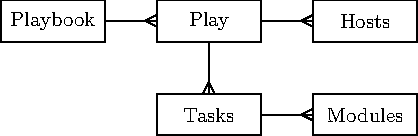
\includegraphics{graph/ansible-0.pdf}
  \caption{Playbook}
  \label{fig:PlaybookRelition}
\end{figure}

该实例的目录结构为:
\begin{verbatim}
# tree playbooks/
playbooks/
|-- group_vars
|   \-- all
|-- hosts
|-- roles
|   \-- common
|       |-- handlers
|       |   \-- main.yml
|       |-- tasks
|       |   \-- main.yml
|       |-- templates
|       |   |-- net-snmp.j2
|       |   |-- ntp.conf.j2
|       |   |-- snmpd.conf.j2
|       |   \-- zypper.repo.j2
|       \-- vars
|           \-- main.yml
\-- site.yml
\end{verbatim}

\begin{verbatim}
# cat playbooks/group_vars/all
---
# Variables listed here are applicable to all host groups
ntpserver: 172.16.25.35
\end{verbatim}

该实例所执行的主机为,
\begin{verbatim}
# cat playbooks/hosts
[bigdata]
172.17.25.31
172.17.25.39
172.17.25.40
\end{verbatim}

\begin{verbatim}
# cat playbooks/common/tasks/main.yml
---
- name: Prepare zyyper repo file
  template: src=zypper.repo.j2 dest=/etc/zypper/repos.d/suse11sp2.repo

- name: Install net-snmp package
  zypper: pkg=net-snmp state=latest

- name: Modify snmp configuration file
  template: src=snmpd.conf.j2 dest=/etc/snmp/snmpd.conf

- name: Modify ntp configuration file
  template: src=ntp.conf.j2 dest=/etc/ntp.conf

- name: Restart ntp service
  shell: /etc/init.d/ntp restart

- name: Enable ntp service
  shell: chkconfig ntp on

- name: Restart snmpd service
  shell: service snmpd restart

- name: Enable snmpd service
  shell: chkconfig snmpd on
\end{verbatim}

\begin{verbatim}
# cat playbooks/common/handlers/main.yml
---
- name: restart snmpd
  service name=snmpd state=restarted enabled=yes

- name: restart ntp
  service: name=ntp state=restarted enabled=yes
\end{verbatim}

snmp日志轮询配置模板,
\begin{verbatim}
# cat playbooks/common/templates/net-snmp.j2
/var/log/net-snmpd.log {
   daily
   compress
   dateext
   maxage 10
   logrotate 10
   size=+1024k
   notifempty
   missingok
   sharedscripts
   postrotate
       /etc/init.d/snmpd reload ||:
	   if [ -x /etc/init.d/snmptrapd ] ; then \
	      /etc/init.d/snmptrapd reload ||: ; \
	   fi
   endscript
}
\end{verbatim}

NTP服务的配置模板,
\begin{verbatim}
# cat playbooks/common/templates/ntp.conf.j2
driftfile /var/lib/ntp/drift/ntp.drift
logfile   /var/log/ntp
server    {{ ntpserver }}
\end{verbatim}

SNMP服务的配置模板,
\begin{verbatim}
# cat playbooks/common/templates/snmpd.conf.j2
rocommunity public
\end{verbatim}

YAST源的配置模板,
\begin{verbatim}
# cat playbooks/common/templates/zypper.repo.j2
name=SUSE-Linux-Enterprise-Server-11-SP2 11.2.2-1.234
enabled=1
autorefresh=1
baseurl=ftp://{{ yastserver }}/
path=/
type=yast2
keeppackages=0
\end{verbatim}

变量文件内容为,
\begin{verbatim}
# cat playbooks/common/vars/main.yml
---
ntpserver: 172.16.25.35
yastserver: 172.16.25.35
\end{verbatim}

该实例的入口文件为,
\begin{verbatim}
# cat playbooks/site.yml
---
- name: apply common configuation to all nodes
  hosts: all
  roles:
  - common
\end{verbatim}

%%% Local Variables:
%%% mode: latex
%%% TeX-master: t
%%% End:
